\newcommand{\LYCORIS}{{\textsc{Lycoris}}\xspace}
\newcommand{\DESYII}{{\mbox{DESY II}}\xspace}
\newcommand{\DIITBF}{{\DESYII Test Beam Facility}\xspace}
\newcommand{\SID}{{SiD}\xspace}
\newcommand{\KPIX}{{KPiX}\xspace}


\section{\KPIX Silicon Tracking}
Most recent update: 2020-05-1135 \\
Contact person: Marty Breidenbach (email: mib@slac.stanford.edu)\\
Contact person: Marcel Stanitzki (email: marcel.stanitzki@desy.de)\\
Contact person: Mengqing Wu (email: mengqing.wu@desy.de)\\




\subsection{Introduction}
The baseline design of the \SID Tracker as presented in the ILC TDR~\cite{Behnke:2013lya} is based on an all-silicon approach.
The main tracker technology of choice is silicon strip sensors arrayed in five nested cylinders in the central
region and four disks following a conical surface with an angle of 5~degrees with respect to the normal to the 
beam line in each of the end regions. The geometry of the end-caps minimizes the material budget to enhance 
forward tracking. The basic building block is a module consisting of a single-sided silicon sensor, two \KPIX readout ASICS and a small Kapton-flex cable
for power delivery and signal distribution.
The sensors have a size of  approximately 10 $\times$ 10 cm$^2$, a strip pitch of \SI{25}{\micro\meter} and a readout pitch of \SI{50}{\micro\meter}.
The end-caps utilizes two modules back-to-back for small angle stereo measurements. 
A drawing of a Tracker module is shown in Figure~\ref{fig:SiliconTrackin:KPiX:module}
\begin{figure}
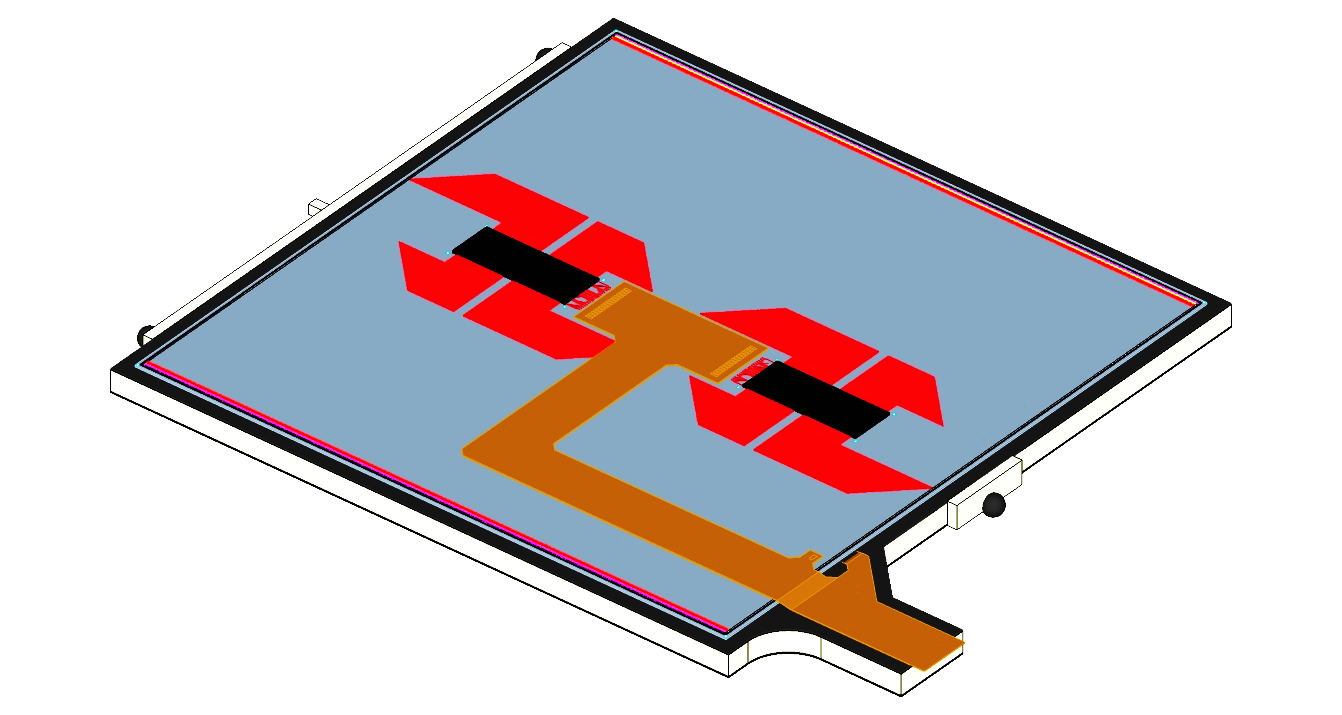
\includegraphics[width=0.49\textwidth]{Tracker/KPIX/Tracker_Module_SiD_Drawing.png}
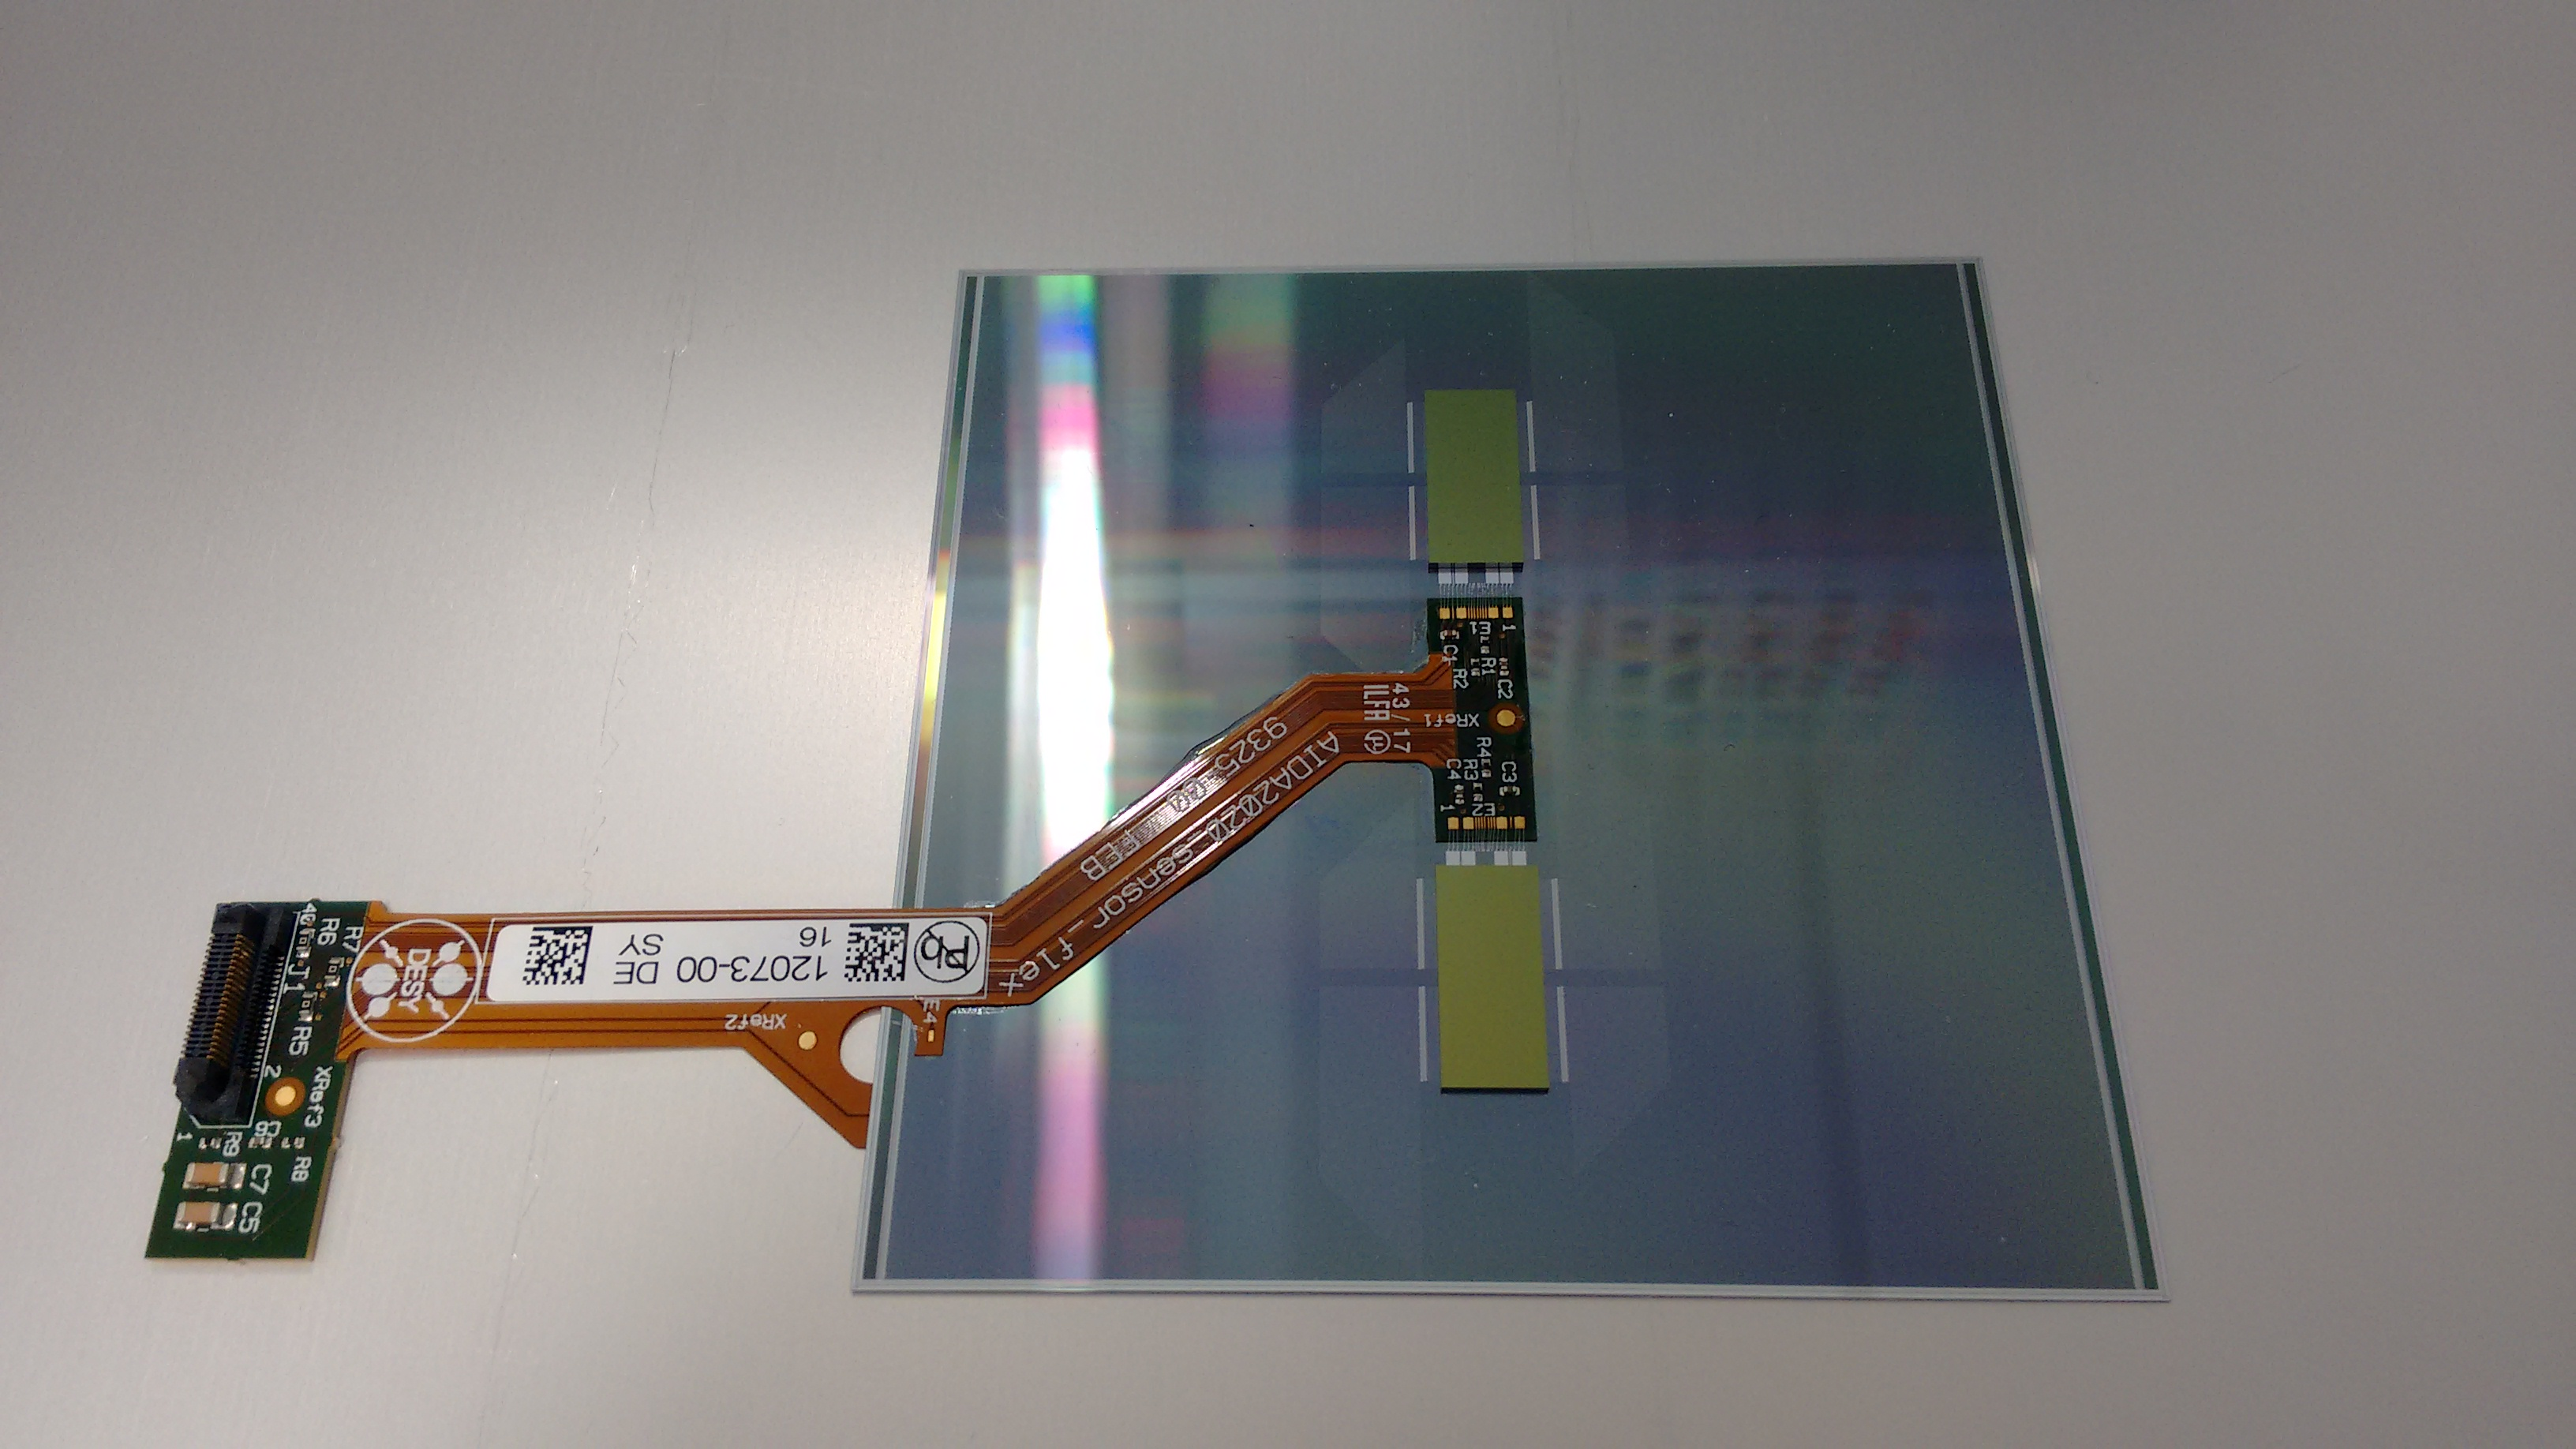
\includegraphics[width=0.49\textwidth]{Tracker/KPIX/Tracker_Module_SiD_Photo.jpg}
\caption{This \SID Tracker Module as foreseen for the baseline \SID Tracker\cite{Behnke:2013lya} with the two \KPIX ASICS and the Kapton-Flex cable 
and a first prototype sensor fully completely assembled at DESY}
\label{fig:SiliconTrackin:KPiX:module}
\end{figure}

The \KPIX ASIC~\cite{6551433}is a 1024 channel ``System on a Chip'' intended for bump bonding 
to large area silicon sensors, enabling low multiple scattering silicon-strip 
tracking and high density Particle Flow calorimetry for \SID at the ILC. 
Each channel consists of a dynamically switchable gain charge amplifier; 
shaping; threshold discrimination; and four sample and hold 
capacitors and four timing registers. The chip permits four  separate measurements of 
amplitude and time of threshold crossing during each train, and amplitude 
digitization and readout during the intertrain period. The dynamic range is from 
sub minimum ionizing particle (MIP) (in \SI{320}{\micro\meter} silicon) to more 
than 2000 MIP. \KPIX also has a calibration system for each channel, servos for 
leakage compensation, ``DC'' reset for asynchronous operation for testing with 
cosmic rays, and polarity inversion for use with GEMs and similar detectors. The 
noise floor is about \SI{0.15}{fC} ($\simeq$ 1000 electrons), and the maximum 
signal is \SI{10}{pC} (utilizing the dynamic range switching). The full dynamic 
range corresponds to 17 bits. \KPIX is manufactured using a \SI{250}{\nano\meter} process at TSMC.

\subsection{Recent Milestones}
ILC related R\&D in the US has been largely unfunded and small efforts are being kept alive. The \KPIX R\&D is such an example of necessary work for \SID.
In the last three years, the R\&D for \KPIX Silicon Tracker has been used to design and build a large-area silicon-strip 
telescope -- called \LYCORIS -- for the \DIITBF~\cite{desytb2018} as part of the Horizon2020-funded AIDA2020~\cite{AIDA2020} project.

Based on the experiences with the first set of sensors, the second generation of sensors was produced by Hamamatsu 
using Au pads for the \KPIX bump-bonds and with a thicker oxide-layer. This was necessary, because the first generation Tracker sensor could not be 
wire-bonded to its (very thin) cable, which was unexpected. It was discovered, that the sensor oxide layer was not strong enough 
to allow wire bonding without damaging the sensor itself.


\subsection{Engineering Challenges}
At this time, \KPIX is seen as the baseline readout system for the tracker and electromagnetic calorimeter. A stack of 13 EMCal sensors with bump bonded \KPIX was assembled for a beam test at SLAC in the summer of 2013. That test discovered that two kinds of cross-talk are significant:
\begin{itemize}
	\item In-time cross talk occurs due to parasitic coupling of traces on metal 2 of the sensor to other pixels. The level of cross-talk increases 
	with the size of the signal, and decreases with increased speed of the front end charge amplifier (meaning increased current and power dissipation).  
	A new sensor design is being developed that uses metal 1 to shield the traces of metal 2, and these ideas will be tested in the next sensor prototype.
	\item Out-of-time cross talk occurs when many pixels are hit and reset simultaneously. The resets collectively cause other pixels to trigger, and a 
	cascade builds up. This uses up all the \KPIX buffers. The root cause of the problem appears to be some internal logic within \KPIX that is not current limited, and will require design modification.
\end{itemize}


Another concern is that the current design of \KPIX has deadtime after a pixel has accepted a trigger. Only the triggered pixel is affected; all the other pixels are available for signals. This deadtime is different from the usual notion of data acquisition deadtime where the entire detector is unavailable, but the correction to the luminosity integral is easy. Finally, the buffer requirement (4 in the current version of \KPIX) is being re-evaluated in \SID simulations. A possible new architecture for \KPIX is in early stages of evaluation.
A small mechanical engineering effort has started to study the structure of the EMCal. The Sid EMCal has emphasized thin gaps between the tungsten layers to minimize the Moliere radius, and this implies that the structure is connected by columns at the vertices of the sensors. The DBD design shows hexagonal sensors, which indeed are the most efficient way of tiling large areas, but no consideration was given to the edges of these arrays. The design is being re-evalutated to optimize the cost-effectiveness over the whole area taking into account geometric efficiencies and total wafer cost.
Tracker sensors are now at IZM for the pad plating and subsequent bonding of \KPIX; they will then go to UCD for cable attachment and testing.


\subsection{Future Plans}
Assuming positive developments with Japan are announced soon, we expect the financial support to improve. It should be noted that
an important effect of the withdrawal of support is that most of the US collaborators have been forced to move to other work.
\begin{itemize}


	\item \KPIX: A new architecture with little (or no) deadtime will be evaluated. A decision will be made to develop this new architecture or incrementally.
	\item improve the existing design.
\subsection{References}

\begin{itemize}
\item \fullcite{lycoris-D15.2}
\item \fullcite{Kraemer:2018qzh}
\item \fullcite{Kraemer:2019xku}
\item \fullcite{Wu:2020jdk}
\end{itemize}
